% !TeX program = xelatex
% 第十五章 多元函数的极限与连续性
\chapter{多元函数的极限与连续性}

到目前为止，我们所讨论的函数都是只有一个自变量的一元函数．它所能描述的只是客观现实中很少的一部分事物的变化规律，而更多的情形需要我们考虑多因素影响下事物的变化规律．例如，矩形的面积依赖于两个量：长和宽；长方体的体积则依赖于三个量：长、宽和高；而空间每一点温度的变化不仅依赖于每一点的位置 $(x,y,z)$，而且还随时间 $t$ 的变化而变化，这时它依赖于四个变量．为此，这一章我们将把一元函数的概念推广到多个自变量的情形，这就是多元函数．从本章起，我们主要研究多元函数的微积分学．

和一元函数一样，极限与连续性是研究多元函数微积分的基础．因此，我们从讲述多元函数的极限与连续性开始，这就是本章的主要内容．

自变量由一个变成多个，一方面，多个要以一个为前提．因此，前面学过的一元函数的极限、连续性与微积分，对以后的学习是必不可少的．读者以后将会不断遇到要用一元结果，或用一元方法的情形．另一方面，由单个（自变量）到多个（自变量），也必然有本质的变化．本质变化之一是，一个自变量作为直线上的点是有（大小）顺序的，而多个自变量，例如二个自变量，作为平面上的点是没有（大小）顺序的．本质变化之二是，对直线上固定的一点，其他点趋向于它只有左右两个方向，十分简单，而平面上则有无穷多个方向（图~\ref{fig:15-1}）．因此，掌握从一元到多元的差异，应该是今后学习中需特别注意的地方．总之，在一元的基础上抓多元，看它们间的异同，是学习以后内容的基本精神．

\begin{figure}[htbp]
\centering
\begin{tikzpicture}[baseline=(current bounding box.center)]
  \fill (0,0) circle (1.6pt);
  \draw[{-Latex}] (-1.3,0.9) .. controls (-0.4,0.5) .. (0,0);
  \draw[{-Latex}] (0,1.4) .. controls (0.3,0.6) .. (0,0);
  \draw[{-Latex}] (1.3,0.9) .. controls (0.5,0.4) .. (0,0);
  \draw[{-Latex}] (1.2,-0.9) .. controls (0.4,-0.5) .. (0,0);
  \draw[{-Latex}] (-1.2,-0.8) .. controls (-0.5,-0.4) .. (0,0);
\end{tikzpicture}\caption{\relax}\label{fig:15-1}
\end{figure}

从一元到二元，是需要许多新思想的，但从二元再到多于二元（$n$ 元），新的思想就不多了，只是形式和计算上会复杂得多．因此，本书后面许多地方只讲二元或三元，$n$ 元的结果需要读者自己写出来．

\section{平面点集}

对一元函数的研究是以实数（即直线上的点）理论为基础的，相应地，对于二元函数，我们需要先研究平面点集．

在平面直角坐标系中，平面上的一个点 $P$ 可以用有序实数对 $(x,y)$ 表示，$x$，$y$ 分别是 $P$ 点的横坐标和纵坐标；反之，任一有序实数对 $(x,y)$ 也对应于平面上的一个点 $P$．因此今后我们对有序实数对和平面上的点 $P$ 不加区别．

平面上两点 $P_{1}(x_{1},y_{1})$ 和 $P_{2}(x_{2},y_{2})$ 之间的距离为
\[
r\left(P_{1},P_{2}\right)=\sqrt{\left(x_{1}-x_{2}\right)^{2}+\left(y_{1}-y_{2}\right)^{2}},
\]
它满足下列性质：
\begin{enumerate}[label=(\arabic*),leftmargin=3em,itemsep=2pt,topsep=2pt]
\item $r(P_{1},P_{2})\geqslant 0$；
\item $r(P_{1},P_{2})=0$ 当且仅当 $P_{1}=P_{2}$；
\item 三角不等式
\[
r\left(P_{1},P_{2}\right)\leqslant r\left(P_{1},P_{3}\right)+r\left(P_{3},P_{2}\right).
\]
\end{enumerate}
这些都是解析几何中已知的基本事实．

平面上的点集可以用集合表示为
\[
E=\left\{(x,y)\mid (x,y)\ \text{满足某性质}\right\}.
\]
例如，二维平面 $\mathbf{R}^{2}$ 的第一象限可表示为
\[
A=\left\{(x,y)\mid x>0,y>0\right\},
\]
而二维平面 $\mathbf{R}^{2}$ 则可表示为
\[
\mathbf{R}^{2}=\left\{(x,y)\mid -\infty<x,y<+\infty\right\}.
\]
又如平面上以 $P_{0}(x_{0},y_{0})$ 点为中心以 $\delta\,(>0)$ 为半径的圆内所有的点可以表示为
\[
\left\{(x,y)\mid \left(x-x_{0}\right)^{2}+\left(y-y_{0}\right)^{2}<\delta^{2}\right\}=\left\{P\mid r\left(P_{0},P\right)<\delta\right\},
\]
称为点 $P_{0}(x_{0},y_{0})$ 的 $\delta$ 圆邻域，或简称圆邻域，记为 $O(P_{0},\delta)$（图~\ref{fig:15-2}）．而点集
\[
\left\{(x,y)\mid \left|x-x_{0}\right|<\delta,\left|y-y_{0}\right|<\delta\right\}
\]
则称为点 $P_{0}(x_{0},y_{0})$ 的 $\delta$ 方邻域，或简称为方邻域，记为 $K(P_{0},\delta)$（图~\ref{fig:15-3}）．它们是直线上常遇到的以 $x_{0}$ 为中心以 $2\delta$ 为长度的开区间
\[
\left(x_{0}-\delta,x_{0}+\delta\right)=\left\{x\mid \left|x-x_{0}\right|<\delta\right\}
\]
到平面的对应物．对应物有两种，这便开始体现了二元的复杂性．但幸好，每个 $P_{0}$ 的 $\delta$ 圆邻域都包含在 $\delta$ 方邻域中，而每个 $\delta$ 方邻域又包含在 $\sqrt{2}\,\delta$ 圆邻域中，即
\[
O\left(P_{0},\delta\right)\subset K\left(P_{0},\delta\right)\subset O\left(P_{0},\sqrt{2}\,\delta\right).
\]
也就是说，任意一个点 $P_{0}$ 的方邻域必包含一个点 $P_{0}$ 的圆邻域，反之亦然（见图~\ref{fig:15-4}）．因此常常不加区别地把圆邻域和方邻域统称为 $P_{0}$ 的邻域．集合
\[
\begin{aligned}
O\left(P_{0},\delta\right)\setminus\left\{P_{0}\right\}&=\left\{(x,y)\mid 0<\left(x-x_{0}\right)^{2}+\left(y-y_{0}\right)^{2}<\delta^{2}\right\},\\
K\left(P_{0},\delta\right)\setminus\left\{P_{0}\right\}&=\left\{(x,y)\mid \left|x-x_{0}\right|<\delta,\left|y-y_{0}\right|<\delta,(x,y)\neq(x_{0},y_{0})\right\}
\end{aligned}
\]
分别称为点 $P_{0}$ 的空心圆邻域和空心方邻域，并分别记为 $O^{*}(P_{0},\delta)$ 和 $K^{*}(P_{0},\delta)$．

\begin{figure}[htbp]
\centering
\begin{tikzpicture}[scale=0.7,baseline=(current bounding box.center)]
  \def\R{1.3}
  \coordinate (P0) at (2.4,2.2);
  \draw[{-Latex}] (0,0) -- (4.3,0) node[below left] {$x$};
  \draw[{-Latex}] (0,0) -- (0,4) node[left] {$y$};
  \node[below left] at (0,0) {$O$};
  \draw[pattern=north east lines] (P0) circle (\R);
  \draw[dashed,thick] (P0) circle (\R);
  \draw[dashed] (P0) -- ++(\R,0) node[midway,above] {$\delta$};
  \fill (P0) circle (1.4pt) node[left] {$P_0$};
\end{tikzpicture}\caption{\relax}\label{fig:15-2}
\end{figure}

\begin{figure}[htbp]
\centering
\begin{tikzpicture}[scale=0.7,baseline=(current bounding box.center)]
  \draw[{-Latex}] (0,0) -- (4.3,0) node[below left] {$x$};
  \draw[{-Latex}] (0,0) -- (0,4) node[left] {$y$};
  \node[below left] at (0,0) {$O$};
  \draw[pattern=north east lines] (1.25,1.05) rectangle (3.55,3.35);
  \draw[dashed,thick] (1.25,1.05) rectangle (3.55,3.35);
  \draw[dashed] (2.4,2.2) -- (3.55,2.2) node[midway,above] {$\delta$};
  \fill (2.4,2.2) circle (1.4pt) node[left] {$P_0$};
\end{tikzpicture}\caption{\relax}\label{fig:15-3}
\end{figure}

\begin{figure}[htbp]
\centering
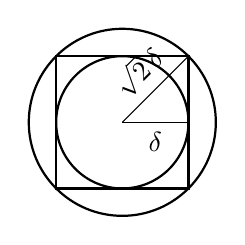
\begin{tikzpicture}[scale=0.8,baseline=(current bounding box.center)]
  \def\s{1.05}
  \draw[thick] (0,0) circle ({\s*1.414});
  \draw[thick] (-\s,-\s) rectangle (\s,\s);
  \draw[thick] (0,0) circle (\s);
  \draw (0,0) -- (\s,0) node[midway,below] {$\delta$};
  \draw (0,0) -- (\s,\s) node[midway,above,sloped] {$\sqrt{2}\,\delta$};
\end{tikzpicture}\caption{\relax}\label{fig:15-4}
\end{figure}

值得指出的是 $K^{*}(P_{0},\delta)$ 不可表示为 $0<\left|x-x_{0}\right|<\delta$，$0<\left|y-y_{0}\right|<\delta$．读者试想想，这是为什么．

设 $E$ 是平面上的点集，下面利用邻域来给出平面上任一点 $P_{0}$ 与点集 $E$ 的关系（见图~\ref{fig:15-5}）．

\begin{enumerate}[label=（\arabic*）,leftmargin=3.2em,itemsep=3pt,topsep=2pt]
\item \textbf{内点}：称 $P_{0}$ 是 $E$ 的内点，如果存在点 $P_{0}$ 的 $\delta$ 邻域完全含于 $E$ 内，即
\[
\exists\,\delta>0,\ \text{使}\ O\left(P_{0},\delta\right)\subset E.
\]
\item \textbf{外点}：称 $P_{0}$ 是 $E$ 的外点，如果存在点 $P_{0}$ 的 $\delta$ 邻域，其中不含 $E$ 的点，即
\[
\exists\,\delta>0,\ \text{使}\ O\left(P_{0},\delta\right)\cap E=\varnothing.
\]
\item \textbf{边界点}：称 $P_{0}$ 是 $E$ 的边界点，如果 $P_{0}$ 点的任意 $\delta$ 邻域中都既有 $E$ 的点，又有非 $E$ 的点，即
\[
\forall \delta>0,\ O\left(P_{0},\delta\right)\cap E\neq\varnothing\ \text{ 且 }\ O\left(P_{0},\delta\right)\setminus E\neq\varnothing.
\]
\item \textbf{聚点}：称 $P_{0}$ 是 $E$ 的聚点，如果 $P_{0}$ 点的任意 $\delta$ 空心邻域中都有 $E$ 的点，即
\[
\forall \delta>0,\ O^{*}\left(P_{0},\delta\right)\cap E\neq\varnothing.
\]
\end{enumerate}

\begin{figure}[htbp]
\centering
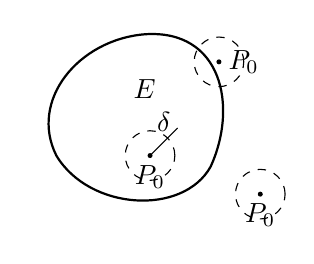
\begin{tikzpicture}[scale=0.7,baseline=(current bounding box.center)]
  \draw[thick] (0.2,1.6) .. controls (1.6,1.7) and (1.9,0.3) .. (1.4,-0.8)
    .. controls (0.9,-1.7) and (-0.8,-1.6) .. (-1.4,-0.6)
    .. controls (-1.9,0.4) and (-1.0,1.5) .. (0.2,1.6) -- cycle;
  \node at (0.2,0.6) {$E$};
  \coordinate (A) at (0.3,-0.6);
  \draw[dashed] (A) circle (0.45);
  \fill (A) circle (1.3pt) node[below] {$P_0$};
  \draw (A) -- ++(0.5,0.5) node[midway,above] {$\delta$};
  \coordinate (B) at (1.55,1.1);
  \draw[dashed] (B) circle (0.45);
  \fill (B) circle (1.3pt) node[right] {$P_0$};
  \coordinate (C) at (2.3,-1.3);
  \draw[dashed] (C) circle (0.45);
  \fill (C) circle (1.3pt) node[below] {$P_0$};
\end{tikzpicture}\caption{\relax}\label{fig:15-5}
\end{figure}

显然，$P_{0}$ 点是 $E$ 的内点、外点或边界点三者必居其一．$E$ 的内点必属于 $E$，$E$ 的外点必不属于 $E$，而 $E$ 的边界点和聚点可能属于 $E$，也可能不属于 $E$．$E$ 的内点是 $E$ 的聚点，外点不是 $E$ 的聚点，边界点可能是 $E$ 的聚点，也可能不是 $E$ 的聚点．

\begin{example}\label{ex:15-1-1}
给定集合 $E=\{(x,y)\mid x^{2}+y^{2}\leqslant 1\}$，则 $E$ 的内点构成的集合为 $\{(x,y)\mid x^{2}+y^{2}<1\}$；$E$ 的外点构成的集合为 $\{(x,y)\mid x^{2}+y^{2}>1\}$；$E$ 的边界点构成的集合为 $\{(x,y)\mid x^{2}+y^{2}=1\}$；$E$ 的聚点全体就是 $E$．
\end{example}

\begin{example}\label{ex:15-1-2}
设 $E=\{(x,y)\mid 0<x<1,0<y<1,x,y\ \text{都是有理数}\}$．则 $E$ 的内点集为空集 $\varnothing$，即 $E$ 没有内点；$E$ 的边界点集为 $\{(x,y)\mid 0\leqslant x\leqslant 1,0\leqslant y\leqslant 1\}$．$E$ 的所有边界点都是 $E$ 的聚点；所有非边界点是 $E$ 的外点．
\end{example}

下面是几种重要的平面点集．

\begin{enumerate}[label=（\arabic*）,leftmargin=3.2em,itemsep=3pt,topsep=2pt]
\item \textbf{开集}\quad 称平面点集 $E$ 是开集，如果 $E$ 的所有点都是内点．
\item \textbf{闭集}\quad 称平面点集 $E$ 是闭集，如果 $E$ 的所有聚点（如果有的话）都属于 $E$．
\item \textbf{连通集}\quad 称 $E$ 是连通集，如果 $E$ 中的任何两点都能用完全含于 $E$ 的由有限条直线段组成的折线连接起来（见图~\ref{fig:15-6}）．
\item \textbf{区域}\quad 连通的开集称为开区域，或简称区域．
\item \textbf{闭区域}\quad 区域连同它的边界点所成的集合称为闭区域．
\end{enumerate}

\begin{figure}[htbp]
\centering
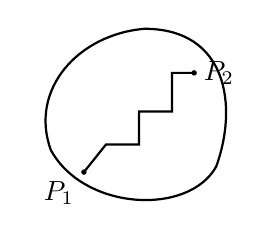
\begin{tikzpicture}[scale=0.7,baseline=(current bounding box.center)]
  \draw[thick] (0.2,1.6) .. controls (1.7,1.6) and (1.9,0.2) .. (1.5,-0.9)
    .. controls (1.0,-1.8) and (-0.9,-1.7) .. (-1.5,-0.6)
    .. controls (-1.9,0.5) and (-1.0,1.5) .. (0.2,1.6) -- cycle;
  \draw[thick] (-0.9,-1.0) -- (-0.5,-0.5) -- (0.1,-0.5) -- (0.1,0.1) -- (0.7,0.1) -- (0.7,0.8) -- (1.1,0.8);
  \fill (-0.9,-1.0) circle (1.4pt) node[below left] {$P_1$};
  \fill (1.1,0.8) circle (1.4pt) node[right] {$P_2$};
\end{tikzpicture}\caption{\relax}\label{fig:15-6}
\end{figure}

例如，邻域 $O(P_{0},\delta)$，$K(P_{0},\delta)$ 是开集，也是区域．集合
\[
\left\{(x,y)\mid \left(x-x_{0}\right)^{2}+\left(y-y_{0}\right)^{2}\leqslant\delta\right\},\quad
\left\{(x,y)\mid \left|x-x_{0}\right|\leqslant\delta,\left|y-y_{0}\right|\leqslant\delta\right\}
\]
都是闭集也是闭区域，其中 $\delta>0$．

例~\ref{ex:15-1-2} 中给出的集合 $E$ 既非开集也非闭集．二维平面 $\mathbf{R}^{2}$ 则既是区域又是闭区域，这是平面点集中除空集外唯一是开集又是闭集的集合．邻域和空心邻域是开集也是区域．

注意：区域总是开集，闭区域总是闭集．但反之未必．例如圆周
\[
\left\{(x,y)\mid x^{2}+y^{2}=\mathbf{R}^{2}\right\}
\]
是闭集，但不是闭区域，因为它没有内点，因而不是由某个开集及其边界构成的（图~\ref{fig:15-7}）．又如
\[
\left\{(x,y)\mid xy>0\right\}
\]
是开集，但不是区域，因为它不连通（图~\ref{fig:15-8}）．

\begin{figure}[htbp]
\centering
\begin{tikzpicture}[scale=0.7,baseline=(current bounding box.center)]
  \draw[{-Latex}] (-2.4,0) -- (2.6,0) node[below left] {$x$};
  \draw[{-Latex}] (0,-2.1) -- (0,2.3) node[left] {$y$};
  \node[below left] at (0,0) {$O$};
  \draw[thick] (0,0) circle (1.7);
  \node[below right] at (1.7,0) {$R$};
\end{tikzpicture}\caption{\relax}\label{fig:15-7}
\end{figure}

\begin{figure}[htbp]
\centering
\begin{tikzpicture}[scale=0.7,baseline=(current bounding box.center)]
  \draw[{-Latex}] (-2.4,0) -- (2.6,0) node[below left] {$x$};
  \draw[{-Latex}] (0,-2.3) -- (0,2.3) node[left] {$y$};
  \node[below left] at (0,0) {$O$};
  \fill[pattern=north east lines] (0.3,0.3) -- (2.0,0.3) -- (0.3,2.0) -- cycle;
  \fill[pattern=north east lines] (-0.3,-0.3) -- (-2.0,-0.3) -- (-0.3,-2.0) -- cycle;
\end{tikzpicture}\caption{\relax}\label{fig:15-8}
\end{figure}

回忆一元函数极限与连续的理论，开区间与闭区间的概念是十分重要的．现在我们看到，区域是直线上开区间在平面的对应物，有界闭区域是直线上闭区间在平面的对应物．把区域、闭区域的多样性与直线的开区间、闭区间相比较，可看到多元问题的确较一元问题复杂得多．

下面给出平面点列的极限概念．

\begin{definition}\label{def:15-1}
设 $\{P_{n}\}$ 是平面上的点列，其中 $P_{n}=(x_{n},y_{n})$．又 $P_{0}=(x_{0},y_{0})$ 是平面上的一点．若对任给的正数 $\varepsilon$，存在正整数 $N$，当 $n>N$ 时，有
\begin{equation}
r\left(P_{n},P_{0}\right)=\sqrt{\left(x_{n}-x_{0}\right)^{2}+\left(y_{n}-y_{0}\right)^{2}}<\varepsilon,
\tag{1}
\end{equation}
则称点列 $\{P_{n}\}$ 收敛到点 $P_{0}$，或称点列 $\{P_{n}\}$ 当 $n$ 趋于无穷时的极限为 $P_{0}$，记为
\[
\lim_{n\to\infty}P_{n}=P_{0}\quad\text{或}\quad P_{n}\to P_{0}\ (n\to\infty).
\]
\end{definition}

（1）式描述的是两点 $P_{n}$ 和 $P_{0}$ 之间的距离小于 $\varepsilon$，这种描述是实数极限 $\lim\limits_{n\to\infty}x_{n}=a$ 的定义中 $\left|x_{n}-a\right|<\varepsilon$ 的直接推广．如果用邻域来描述，则（1）式等价于
\[
P_{n}\in O\left(P_{0},\varepsilon\right).
\]
因此平面上点列 $\{P_{n}\}$ 收敛到 $P_{0}$ 的几何意义是：对 $P_{0}$ 的任意邻域 $O(P_{0},\varepsilon)$，至多有点列的有限项 $P_{1},\cdots,P_{N}$ 不在邻域 $O(P_{0},\varepsilon)$ 内，其余的 $P_{n}$ 全部落在 $P_{0}$ 的邻域 $O(P_{0},\varepsilon)$ 内．

不难证明下列各式是等价的，请读者写出它们的证明．

\begin{enumerate}[label=(\roman*),leftmargin=3.2em,itemsep=2pt,topsep=2pt]
\item $\displaystyle\lim_{n\to\infty}P_{n}=P_{0}$；
\item $\displaystyle\lim_{n\to\infty}r(P_{n},P_{0})=0$；
\item $\displaystyle\lim_{n\to\infty}x_{n}=x_{0}$，且 $\displaystyle\lim_{n\to\infty}y_{n}=y_{0}$．
\end{enumerate}

注意到（ii）和（iii）就是实数列的极限，因此上述等价性使得我们可以方便地应用实数的极限理论．例如由实数列极限的唯一性立即可知平面点列的极限若存在则是唯一的．

\begin{figure}[htbp]
\centering
\begin{tikzpicture}[scale=0.7,baseline=(current bounding box.center)]
  \def\R{1.3}
  \coordinate (P0) at (2.4,2.2);
  \draw[{-Latex}] (0,0) -- (4.3,0) node[below left] {$x$};
  \draw[{-Latex}] (0,0) -- (0,4) node[left] {$y$};
  \node[below left] at (0,0) {$O$};
  \draw[pattern=north east lines] (P0) circle (\R);
  \draw[dashed,thick] (P0) circle (\R);
  \draw[dashed] (P0) -- ++(\R,0) node[midway,above] {$\varepsilon$};
  \fill (P0) circle (1.4pt) node[left] {$P_0$};
\end{tikzpicture}\caption{\relax}\label{fig:15-9}
\end{figure}

\begin{example}\label{ex:15-1-3}
设 $P_{n}=\left\{\dfrac{1}{n},\sin\dfrac{1}{n}\right\}$，$P_{0}=(0,0)$，则 $\lim\limits_{n\to\infty}P_{n}=P_{0}$．设 $P_{n}=\left\{\left(1+\dfrac{1}{n}\right)^{n},\cos\dfrac{1}{n}\right\}$，$P_{0}=(\mathrm{e},1)$，则 $\lim\limits_{n\to\infty}P_{n}=P_{0}$．
\end{example}

实数的连续性、完备性和有界闭集的紧致性（前面我们只讲过闭区间）是一元函数微积分的基础．连续性涉及实数的顺序，这里不多讲了．下面我们将完备性和紧致性推广到二维情形，它们同样是二元函数微积分的基础．

\begin{theorem}[柯西收敛原理]\label{thm:15-1}
平面点列 $\{P_{n}\}$ 收敛的充分必要条件是：对任给的正数 $\varepsilon$，存在正整数 $N$，当 $n$，$m>N$ 时，有
\begin{equation}
r\left(P_{n},P_{m}\right)<\varepsilon.
\tag{2}
\end{equation}
\end{theorem}

\begin{proof}
必要性．设平面点列 $\{P_{n}\}$ 收敛于 $P_{0}$，由极限定义知，对任给的 $\varepsilon>0$，存在 $N$，当 $n>N$ 时有
\[
r\left(P_{n},P_{0}\right)<\frac{\varepsilon}{2}.
\]
于是由距离的三角不等式，当 $n$，$m>N$ 时有
\[
r\left(P_{n},P_{m}\right)\leqslant r\left(P_{n},P_{0}\right)+r\left(P_{0},P_{m}\right)<\frac{\varepsilon}{2}+\frac{\varepsilon}{2}=\varepsilon.
\]

充分性．设 $P_{n}(x_{n},y_{n})$ 满足已知条件，即对任给的 $\varepsilon>0$，存在 $N$，当 $n$，$m>N$ 时，有
\[
r\left(P_{n},P_{m}\right)=\sqrt{\left(x_{n}-x_{m}\right)^{2}+\left(y_{n}-y_{m}\right)^{2}}<\varepsilon,
\]
从而有
\[
\left|x_{n}-x_{m}\right|<\varepsilon,\quad\left|y_{n}-y_{m}\right|<\varepsilon.
\]
由数列极限的柯西收敛原理知，数列 $\{x_{n}\}$ 和 $\{y_{n}\}$ 都收敛，设分别收敛到 $x_{0},y_{0}$：$x_{n}\to x_{0}$，$y_{n}\to y_{0}$．因此 $P_{n}(x_{n},y_{n})\to P_{0}(x_{0},y_{0})\ (n\to\infty)$，故平面点列 $\{P_{n}\}$ 收敛．定理~\ref{thm:15-1} 证完．
\end{proof}

对比第九章 §3 数列的柯西收敛原理的证明，我们看到，这里必要性的证明，用的是数列情形的证明方法，而充分性的证明则用的是数列情形的结果．

\begin{definition}\label{def:15-2}
称平面点列为有界的，如果存在正数 $M$，使
\[
r\left(P_{n},O\right)\leqslant M.
\]
\end{definition}

容易看出，点列 $\{P_{n}(x_{n},y_{n})\}$ 有界，当且仅当数列 $\{x_{n}\}$，$\{y_{n}\}$ 均有界．

\begin{theorem}[波尔察诺--魏尔斯特拉斯致密性定理]\label{thm:15-2}
若点列 $\{P_{n}\}$ 有界，则 $\{P_{n}\}$ 必有收敛子列．
\end{theorem}

\begin{proof}
相继地用两次实数列的致密性定理．已知点列 $\{P_{n}\}$ 有界，$P_{n}=(x_{n},y_{n})$．这时实数列 $\{x_{n}\}$ 和 $\{y_{n}\}$ 有界．因此 $\{x_{n}\}$ 有收敛子列 $\{x_{n_{k}}\}$，即 $x_{n_{k}}\to x_{0}\ (k\to\infty)$．由相应的实数列 $\{y_{n_{k}}\}$ 有界，知它有收敛子列 $\{y_{n_{k_{l}}}\}$，即 $y_{n_{k_{l}}}\to y_{0}\ (l\to\infty)$，而对应的 $\{x_{n_{k_{l}}}\}$ 是 $\{x_{n_{k}}\}$ 的子列，因此 $x_{n_{k_{l}}}\to x_{0}\ (l\to\infty)$．于是 $P_{n_{k_{l}}}=(x_{n_{k_{l}}},y_{n_{k_{l}}})$ 构成的平面点列 $\{P_{n_{k_{l}}}\}$ 是 $\{P_{n}\}$ 的子列，它有极限 $P_{0}(x_{0},y_{0})$，定理~\ref{thm:15-2} 证完．
\end{proof}

定理~\ref{thm:15-2} 的证明，用的是一元的结果．

\begin{theorem}[矩形套定理]\label{thm:15-3}
设 $D_{n}=\left\{(x,y)\mid a_{n}\leqslant x\leqslant b_{n},c_{n}\leqslant y\leqslant d_{n}\right\}$ 是平面上的闭矩形序列（图~\ref{fig:15-10}），满足
\[
\begin{aligned}
1^{\circ}\quad & a_{n}\leqslant a_{n+1}\leqslant b_{n+1}\leqslant b_{n},\ c_{n}\leqslant c_{n+1}\leqslant d_{n+1}\leqslant d_{n},\ n=1,2,\cdots;\\
2^{\circ}\quad & b_{n}-a_{n}\to 0\ \ (n\to\infty),\ d_{n}-c_{n}\to 0\ \ (n\to\infty).
\end{aligned}
\]
则存在唯一的一点 $P_{0}(x_{0},y_{0})$，使得 $P_{0}\in\bigcap\limits_{n=1}^{\infty}D_{n}$，即
\[
a_{n}\leqslant x_{0}\leqslant b_{n},\quad c_{n}\leqslant y_{0}\leqslant d_{n},\quad n=1,2,\cdots.
\]
\end{theorem}

\begin{figure}[htbp]
\centering
\begin{tikzpicture}[scale=0.7,baseline=(current bounding box.center)]
  \draw[{-Latex}] (0,0) -- (4.6,0) node[below left] {$x$};
  \draw[{-Latex}] (0,0) -- (0,4.0) node[left] {$y$};
  \node[below left] at (0,0) {$O$};
  \draw[thick] (0.6,0.6) rectangle (4.2,3.4);
  \draw[thick] (1.0,1.0) rectangle (3.6,2.9);
  \draw[thick] (1.7,1.6) rectangle (2.9,2.4);
  \draw[dashed] (0.6,0) -- (0.6,0.6);
  \draw[dashed] (1.0,0) -- (1.0,1.0);
  \draw[dashed] (3.6,0) -- (3.6,2.9);
  \draw[dashed] (4.2,0) -- (4.2,3.4);
  \draw[dashed] (0,0.6) -- (0.6,0.6);
  \draw[dashed] (0,1.0) -- (1.0,1.0);
  \draw[dashed] (0,2.9) -- (3.6,2.9);
  \draw[dashed] (0,3.4) -- (4.2,3.4);
  \node[below] at (0.6,0) {$a_1$};
  \node[below] at (1.0,0) {$a_2$};
  \node[below] at (3.6,0) {$b_2$};
  \node[below] at (4.2,0) {$b_1$};
  \node[left] at (0,3.4) {$d_1$};
  \node[left] at (0,2.9) {$d_2$};
  \node[left] at (0,1.0) {$c_2$};
  \node[left] at (0,0.6) {$c_1$};
\end{tikzpicture}\caption{\relax}\label{fig:15-10}
\end{figure}

\begin{proof}
只要对区间套 $\{[a_{n},b_{n}]\}$ 和 $\{[c_{n},d_{n}]\}$ 分别用区间套定理即可．
\end{proof}

最后我们用矩形套定理来证明平面上的有限覆盖定理．先给出覆盖的定义．

\begin{definition}\label{def:15-3}
设 $\zeta$ 是由开集构成的集族．称 $\zeta$ 是集合 $E$ 的一个覆盖，如果对任意点 $P\in E$，存在开集 $G\in\zeta$，使 $P\in G$，即 $E\subset\bigcup\limits_{G\in\zeta}G$．
\end{definition}

\begin{theorem}[博雷尔有限覆盖定理]\label{thm:15-4}
设 $E$ 是平面上的有界闭集，$\zeta$ 是 $E$ 的一个覆盖，则 $\zeta$ 中存在有限个开集 $G_{1},G_{2},\cdots,G_{n}$，使 $E\subset\bigcup\limits_{i=1}^{n}G_{i}$．
\end{theorem}

定理~\ref{thm:15-4} 说的是有界闭集 $E$ 的任何覆盖，必存在有限子覆盖．定理的证明很难用一元的结果，只好用一元的方法．

\begin{proof}[定理~\ref{thm:15-4} 的证明]
用反证法．已知 $E$ 是平面上的有界闭集，因此存在闭矩形
\[
D=\left\{(x,y)\mid a\leqslant x\leqslant b,c\leqslant y\leqslant d\right\},
\]
使 $E$ 含于 $D$．设 $E$ 不能被 $\zeta$ 中有限个开集所覆盖．用 $D$ 的对边中点的连线
\[
x=\frac{a+b}{2},\quad y=\frac{c+d}{2}
\]
把矩形 $D$ 分成四个相等的闭矩形，则其中至少有一个闭矩形，它包含 $E$ 的部分不能被 $\zeta$ 中有限个开集所覆盖，记这个闭矩形为
\[
D_{1}=\left\{(x,y)\mid a_{1}\leqslant x\leqslant b_{1},c_{1}\leqslant y\leqslant d_{1}\right\}.
\]
再用 $D_{1}$ 对边中点的连线把矩形 $D_{1}$ 分成四个相等的闭矩形，其中至少有一个闭矩形，它包含 $E$ 的部分不能被 $\zeta$ 中有限个开集所覆盖，记这个闭矩形为 $D_{2}$．如此继续下去，得闭矩形序列 $\{D_{n}\}$，满足
\[
\begin{aligned}
1^{\circ}\quad & D_{n}\supseteq D_{n+1},\ n=1,2,\cdots;\\
2^{\circ}\quad & \text{矩形的边长分别为}\ b_{n}-a_{n},\ d_{n}-c_{n},\ \text{且}\\
& b_{n}-a_{n}=\frac{b-a}{2^{n}}\to 0,\quad d_{n}-c_{n}=\frac{d-c}{2^{n}}\to 0\ \ (n\to\infty);\\
3^{\circ}\quad & D_{n}\cap E\ \text{不能被}\ \zeta\ \text{中有限个开集所覆盖}.
\end{aligned}
\]
由矩形套定理，存在唯一的点 $P_{0}(x_{0},y_{0})$ 使得 $P_{0}\in\bigcap\limits_{n=1}^{\infty}D_{n}$，又因为 $D_{n}\cap E\neq\varnothing$，则存在 $P_{n}(x_{n},y_{n})\in D_{n}\cap E$，即
\[
a_{n}\leqslant x_{n}\leqslant b_{n},\quad c_{n}\leqslant y_{n}\leqslant d_{n},\quad n=1,2,\cdots,
\]
而且
\[
\lim_{n\to\infty}a_{n}=\lim_{n\to\infty}b_{n}=x_{0},\quad \lim_{n\to\infty}c_{n}=\lim_{n\to\infty}d_{n}=y_{0},
\]
故
\[
\lim_{n\to\infty}x_{n}=x_{0},\quad\lim_{n\to\infty}y_{n}=y_{0}.
\]
由于 $E$ 是闭集，故 $P_{0}(x_{0},y_{0})\in E$．根据 $\zeta$ 是 $E$ 的覆盖，则存在 $G\in\zeta$，使 $P_{0}\in G$．因为 $G$ 是开集，所以存在 $P_{0}$ 的 $\delta$ 邻域
\[
\Delta=\left\{(x,y)\mid \left|x-x_{0}\right|<\delta,\left|y-y_{0}\right|<\delta\right\},
\]
使得 $\Delta\subset G$．注意到 $\{a_{n}\}$ 和 $\{b_{n}\}$ 的极限为 $x_{0}$，$\{c_{n}\}$ 和 $\{d_{n}\}$ 的极限为 $y_{0}$，从而存在 $N$，当 $n>N$ 时有
\[
x_{0}-\delta<a_{n}<b_{n}<x_{0}+\delta,\quad y_{0}-\delta<c_{n}<d_{n}<y_{0}+\delta,
\]
所以 $D_{n}\subset\Delta\subset G$，即 $D_{n}\cap E$ 被 $\zeta$ 的一个集 $G$ 所覆盖．这与前面的性质 $3^{\circ}$ 矛盾．因此 $\zeta$ 中必有有限个开集覆盖 $E$．定理~\ref{thm:15-4} 证完．
\end{proof}

回忆第九章 §2，知定理~\ref{thm:15-4} 说明平面上有界闭集是紧致的．注意与直线上的有限覆盖定理一样，定理中 $E$ 是有界和闭的条件缺一不可．事实上取
\[
E=\left\{(x,y)\mid x^{2}+y^{2}<1\right\},
\]
则 $E$ 是有界的，但非闭．令
\[
G_{n}=\left\{(x,y)\mid x^{2}+y^{2}<\left(1-\frac{1}{n}\right)^{2}\right\}.
\]
显然 $\zeta=\left\{G_{n}\mid n=2,3,\cdots\right\}$ 是 $E$ 的覆盖，但不存在 $E$ 的有限子覆盖．又如取
\[
E=\left\{(x,y)\mid x\geqslant 0,y\geqslant 0\right\},
\]
则 $E$ 是闭集，但无界．取
\[
G_{n}=\left\{(x,y)\mid x^{2}+y^{2}<n^{2}\right\}.
\]
显然 $\zeta=\left\{G_{n}\mid n=1,2,\cdots\right\}$ 是 $E$ 的覆盖，但不存在 $E$ 的有限子覆盖．

\begin{xiti}
\item 设 $\{P_{n}=(x_{n},y_{n})\}$ 是平面点列，$P_{0}=(x_{0},y_{0})$ 是平面上的点．证明 $\lim\limits_{n\to\infty}P_{n}=P_{0}$ 的充要条件是 $\lim\limits_{n\to\infty}x_{n}=x_{0}$，且 $\lim\limits_{n\to\infty}y_{n}=y_{0}$．
\item 设平面点列 $\{P_{n}\}$ 收敛，证明 $\{P_{n}\}$ 有界．
\item 判别下列平面点集哪些是开集、闭集、有界集或区域，并分别指出它们的聚点：
\begin{ziti}
\item $E=\left\{(x,y)\mid y<x^{2}\right\}$；
\item $E=\left\{(x,y)\mid x^{2}+y^{2}\neq 1\right\}$；
\item $E=\left\{(x,y)\mid xy\neq 0\right\}$；
\item $E=\left\{(x,y)\mid xy=0\right\}$；
\item $E=\left\{(x,y)\mid 0\leqslant y\leqslant 2,2y\leqslant x\leqslant 2y+2\right\}$；
\item $E=\left\{(x,y)\mid y=\sin\dfrac{1}{x},x>0\right\}$；
\item $E=\left\{(x,y)\mid x^{2}+y^{2}=1\ \text{或}\ y=0,0\leqslant x\leqslant 1\right\}$；
\item $E=\left\{(x,y)\mid x,y\ \text{均为整数}\right\}$．
\end{ziti}
\item 设 $F$ 是闭集，$G$ 是开集，证明 $F\setminus G$ 是闭集，$G\setminus F$ 是开集．
\item 证明开集的余集是闭集．
\item 设 $E$ 是平面点集．证明 $P_{0}$ 是 $E$ 的聚点的充要条件是 $E$ 中存在点列 $\{P_{n}\}$，满足 $P_{n}\neq P_{0}\ (n=1,2,\cdots)$ 且 $\lim\limits_{n\to\infty}P_{n}=P_{0}$．
\item 用平面上的有限覆盖定理证明平面上的致密性定理．
\item 用平面上的致密性定理证明平面点列的柯西收敛原理．
\item 设 $E$ 是平面点集，如果集合 $E$ 的任一覆盖都有有限子覆盖，则称 $E$ 是紧集．证明紧集是有界闭集．
\item 设 $E$ 是平面上的有界闭集，$d(E)$ 是 $E$ 的直径，即
\[
d(E)=\sup_{P^{\prime},P^{\prime\prime}\in E}r\left(P^{\prime},P^{\prime\prime}\right).
\]
求证：存在 $P_{1}$，$P_{2}\in E$，使得 $r(P_{1},P_{2})=d(E)$．
\item 仿照平面点集，叙述 $n$ 维欧氏空间中点集的有关概念（如邻域、极限、开集、聚点、闭集、区域、有界以及一些基本定理等）．
\item 叙述并证明三维空间的波尔察诺--魏尔斯特拉斯致密性定理．
\end{xiti}

\section{多元函数的极限与连续性}

\subsection{多元函数的概念}

仿照一元函数的情形，我们先给出二元函数的定义．

\begin{definition}\label{def:15-4}
设 $E$ 是平面点集．如果存在对应关系 $f$，使得对任意的 $(x,y)\in E$，按这个对应关系 $f$，有唯一的实数 $u$ 与之对应，则称 $f$ 为定义在 $E$ 上的二元函数，记为
\[
\begin{aligned}
f\colon E&\to\mathbf{R},\\
(x,y)&\to u=f(x,y).
\end{aligned}
\]
称 $E$ 为函数 $f$ 的定义域，$x$、$y$ 称为函数 $f$ 的自变量，而 $u$ 则称为因变量．$u=f(x,y)$ 是函数 $f$ 在 $(x,y)$ 点所对应的函数值，全体函数值的集合 $f(E)$ 称为函数 $f$ 的值域．
\end{definition}

在数学分析中，为了方便，我们也常把二元函数记为
\[
u=f(x,y),\quad(x,y)\in E
\]
或
\[
u=f(P),\quad P\in E.
\]

\begin{example}\label{ex:15-2-1}
半径为 $r$，高为 $h$ 的圆柱体的体积 $u$ 可表为
\[
u=\pi r^{2}h.
\]
根据实际意义，它的定义域是 $r>0$，$h>0$，值域是 $(0,+\infty)$．
\end{example}

\begin{example}\label{ex:15-2-2}
函数 $u=\sqrt{R^{2}-\left(x^{2}+y^{2}\right)}$ 的定义域是 $x^{2}+y^{2}\leqslant R^{2}$，值域是 $[0,R]$．
\end{example}

\begin{example}\label{ex:15-2-3}
函数 $u=\arcsin\dfrac{x}{a}+\arcsin\dfrac{y}{b}$ 的定义域是 $-a\leqslant x\leqslant a$，$-b\leqslant y\leqslant b$，值域是 $[-\pi,\pi]$．
\end{example}

在一元函数的微积分中，几何图形给了我们很直观的认识，对分析起着重要的作用．二元函数也是如此，几何直观仍是十分重要的．下面给出二元函数的几何表示．

空间点集
\[
\left\{(x,y,z)\mid z=f(x,y),(x,y)\in E\right\}
\]
称为函数 $z=f(x,y)$ 的图形．一般来说它构成一块空间曲面，定义域 $E$ 就是这块曲面在 $Oxy$ 平面上的投影．曲面的特点是，过定义域每一点平行于 $z$ 轴的直线只与曲面相交于一点．

例~\ref{ex:15-2-2} 中函数的图形是以原点为中心以 $R$ 为半径的上半球面，如图~\ref{fig:15-11} 所示．

从解析几何知道，$z=x^{2}+y^{2}$ 的图形是椭圆抛物面（图~\ref{fig:15-12}）．

\begin{figure}[htbp]
\centering
\begin{minipage}[c]{0.48\textwidth}\centering
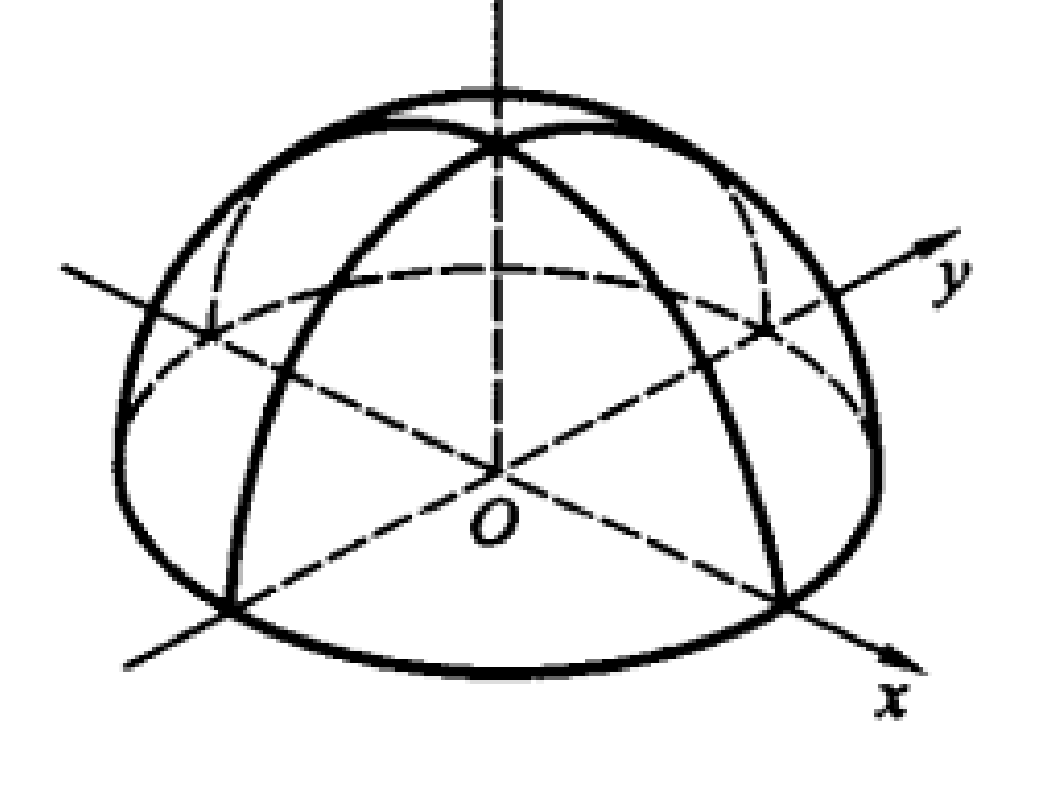
\includegraphics[width=0.72\textwidth]{work/figures/fig15-11}\caption{\relax}\label{fig:15-11}
\end{minipage}\hfill
\begin{minipage}[c]{0.48\textwidth}\centering
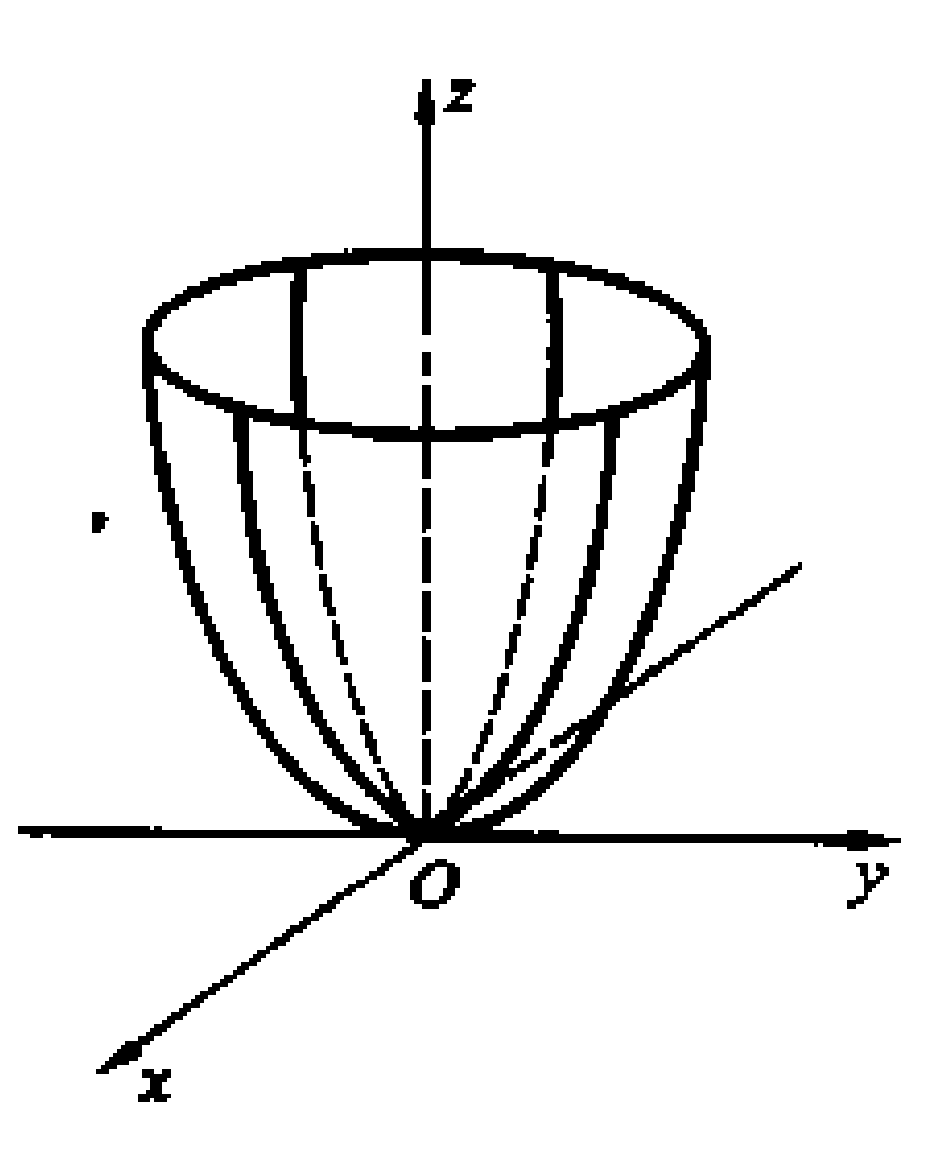
\includegraphics[width=0.72\textwidth]{work/figures/fig15-12}\caption{\relax}\label{fig:15-12}
\end{minipage}
\end{figure}

$z=\sqrt{x^{2}+y^{2}}$ 的图形是锥面（图~\ref{fig:15-13}）．而 $z=xy$ 的图形是双曲抛物面（图~\ref{fig:15-14}）．

\begin{figure}[htbp]
\centering
\begin{minipage}[c]{0.42\textwidth}\centering
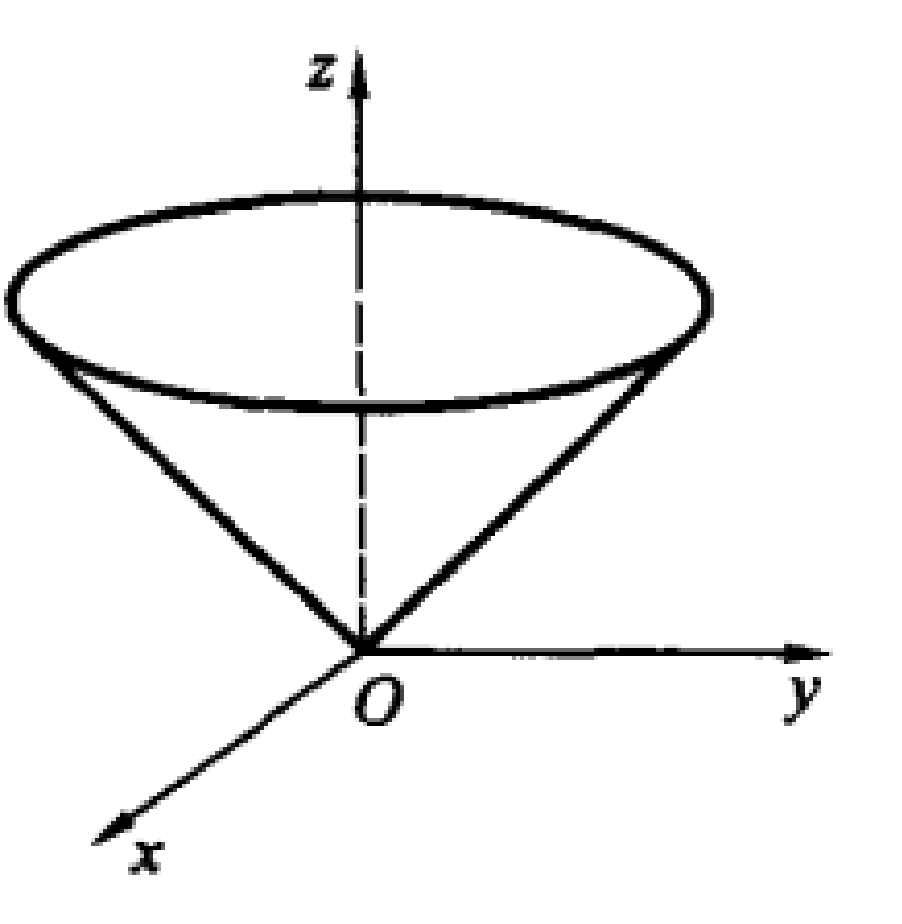
\includegraphics[width=0.72\textwidth]{work/figures/fig15-13}\caption{\relax}\label{fig:15-13}
\end{minipage}\hfill
\begin{minipage}[c]{0.55\textwidth}\centering
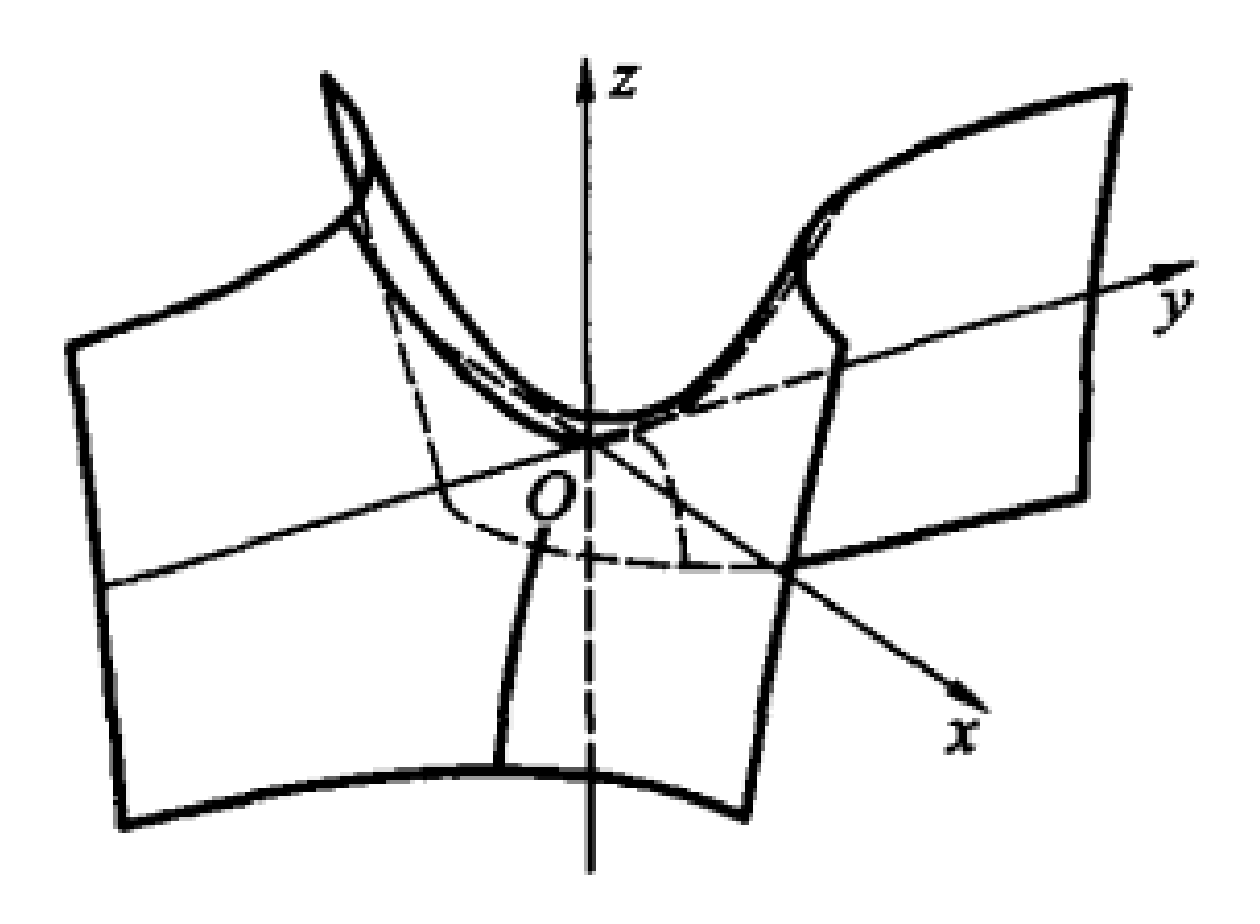
\includegraphics[width=0.9\textwidth]{work/figures/fig15-14}\caption{\relax}\label{fig:15-14}
\end{minipage}
\end{figure}

二元函数的定义很容易推广到多元函数的情形，只要在定义中将二元有序数对 $(x,y)$ 改为 $n$ 元有序数组 $(x_{1},x_{2},\cdots,x_{n})$ 即可．在此不详细叙述．我们简记 $n$ 元函数为
\[
u=f(x_{1},x_{2},\cdots,x_{n}),\ (x_{1},x_{2},\cdots,x_{n})\in E,
\]
或
\[
u=f(P),\ P\in E,
\]
其中
\[
E\subset\mathbf{R}^{n}=\left\{\left(x_{1},x_{2},\cdots,x_{n}\right)\mid -\infty<x_{i}<+\infty,i=1,2,\cdots,n\right\}.
\]
后一种写法是点的形式，它在形式上使多元函数与一元函数保持一致，以便于用类比的方法，把低维的（一元或二元的）结果及研究方法推广到高维．

\subsection{二元函数的极限}

\begin{definition}\label{def:15-5}
设 $f$ 在 $P_{0}(x_{0},y_{0})$ 的某个空心邻域内有定义，$A$ 是一个确定的数．如果对任给的 $\varepsilon>0$，存在 $\delta>0$，使得当 $0<r(P,P_{0})<\delta$ 时，有
\[
\left|f(P)-A\right|<\varepsilon,
\]
那么称 $A$ 是二元函数 $f$ 当 $P\to P_{0}$ 时的极限，记为
\[
\lim_{P\to P_{0}}f(P)=A,
\]
或
\[
\lim_{\substack{x\to x_{0}\\ y\to y_{0}}}f(x,y)=A.
\]
\end{definition}

注意到 $0<r(P,P_{0})<\delta$ 等价于 $P\in O^{*}(P_{0},\delta)$，而 $\left|f(P)-A\right|<\varepsilon$ 等价于 $f(P)\in(A-\varepsilon,A+\varepsilon)=O(A,\varepsilon)$（直线上的邻域）．因此，上述定义又可以用邻域的语言叙述为：对任给的 $\varepsilon>0$，存在 $\delta>0$，只要 $P\in O^{*}(P_{0},\delta)$，就有
\[
f(P)\in O(A,\varepsilon).
\]
由于圆邻域和方邻域可以互相包含，因此上述定义也可叙述为：对任给的 $\varepsilon>0$，存在 $\delta>0$，只要 $P\in K^{*}(P_{0},\delta)$，就有
\[
f(P)\in O(A,\varepsilon).
\]
但在解题时，还是用下述的不等式说法方便：
\[
\lim_{\substack{x\to x_{0}\\ y\to y_{0}}}f(x,y)=A,
\]
当且仅当对任给的 $\varepsilon>0$，存在 $\delta>0$，只要 $0<\sqrt{\left(x-x_{0}\right)^{2}+\left(y-y_{0}\right)^{2}}<\delta$，就有
\[
\left|f(x,y)-A\right|<\varepsilon.
\]
或当且仅当对任给的 $\varepsilon>0$，存在 $\delta>0$，只要 $\left|x-x_{0}\right|<\delta$，$\left|y-y_{0}\right|<\delta$，$(x,y)\neq(x_{0},y_{0})$，有
\[
\left|f(x,y)-A\right|<\varepsilon.
\]

\begin{example}\label{ex:15-2-4}
设 $f(x,y)=xy\dfrac{x^{2}-y^{2}}{x^{2}+y^{2}}$，证明 $\lim\limits_{\substack{x\to0\\y\to0}}f(x,y)=0$．
\end{example}

\begin{proof}[证明]
因为
\[
\begin{aligned}
\left|f(x,y)-0\right|&=\left|\,xy\,\dfrac{x^{2}-y^{2}}{x^{2}+y^{2}}\right|\leqslant\left|\,xy\,\right|\dfrac{x^{2}+y^{2}}{x^{2}+y^{2}}\\
&=\left|\,xy\right|\leqslant\dfrac{x^{2}+y^{2}}{2},
\end{aligned}
\]
所以对任给的 $\varepsilon>0$，要 $\left|f(x,y)-0\right|<\varepsilon$，只要 $\dfrac{x^{2}+y^{2}}{2}<\varepsilon$．取 $\delta=\sqrt{2\varepsilon}$，则当 $0<\sqrt{x^{2}+y^{2}}<\delta$ 时，有
\[
\left|f(x,y)-0\right|\leqslant\dfrac{x^{2}+y^{2}}{2}<\varepsilon.
\]
也可以取 $\delta=\sqrt{\varepsilon}$，则只要 $\left|x\right|<\delta$，$\left|y\right|<\delta$，$(x,y)\neq(0,0)$，就有
\[
\left|f(x,y)-0\right|\leqslant\left|xy\right|<\delta^{2}=\varepsilon.
\]
回忆一元的情形，知道这里用的是“适当放大法”．
\end{proof}

二元函数极限 $\lim\limits_{P\to P_{0}}f(P)=A$ 的几何意义是：对任给的 $\varepsilon>0$，必存在点 $P_{0}$ 的 $\delta$ 空心邻域 $O^{*}(P_{0},\delta)$，使得经过 $f$ 的对应，空心邻域中所有点的像全部落在区间 $(A-\varepsilon,A+\varepsilon)$ 之中（图~\ref{fig:15-15}），即
\[
f\left(O^{*}\left(P_{0},\delta\right)\right)\subset\left(A-\varepsilon,A+\varepsilon\right).
\]

\begin{figure}[htbp]
\centering
\begin{tikzpicture}[scale=0.72,baseline=(current bounding box.center)]
  \draw[thick] (0,2.2) .. controls (1.6,2.3) and (2.0,1.2) .. (1.7,0.4)
    .. controls (1.5,-0.2) and (0.5,0.1) .. (0.2,-0.4)
    .. controls (-0.1,-1.0) and (-1.3,-0.9) .. (-1.5,0.0)
    .. controls (-1.7,1.0) and (-1.0,2.1) .. (0,2.2) -- cycle;
  \node at (1.1,1.4) {$\Omega$};
  \coordinate (P0) at (-0.3,1.2);
  \draw[thick] (P0) circle (0.5);
  \fill (P0) circle (1.4pt) node[above right] {$P_0$};
  \draw (P0) -- ++(180:0.5) node[midway,above] {$\delta$};
  \draw[{-Latex},thick] (0.2,-0.4) .. controls (0.5,-1.0) .. (0.9,-1.4) node[midway,right] {$f$};
  \draw (-0.6,-1.6) -- (2.6,-1.6);
  \draw (-0.2,-1.75) -- (-0.2,-1.45);
  \draw (2.0,-1.75) -- (2.0,-1.45);
  \draw (0.9,-1.75) -- (0.9,-1.45);
  \fill (0.9,-1.6) circle (1.4pt) node[below] {$A$};
  \node[below] at (-0.2,-1.75) {$A-\varepsilon$};
  \node[below] at (2.0,-1.75) {$A+\varepsilon$};
\end{tikzpicture}\caption{\relax}\label{fig:15-15}
\end{figure}

借助于几何直观，我们可以看到平面上的点 $P\to P_{0}$ 的意义远比直线上 $x\to x_{0}$ 要复杂得多．在直线上，$x\to x_{0}$ 只有左、右两个方向，而在平面上 $P\to P_{0}$ 的方向有无穷多个，且路径也有无穷多种（图~\ref{fig:15-16}）．例如 $P$ 点可沿直线趋于 $P_{0}$，也可沿曲线趋于 $P_{0}$．在极限定义中，只要 $P$ 与 $P_{0}$ 充分接近，不管按何种方向何种途径接近，都有 $f(P)$ 与 $A$ 之差任意小．这就说明了二元函数极限要比一元函数极限复杂许多．

\begin{figure}[htbp]
\centering
\begin{tikzpicture}[scale=0.7,baseline=(current bounding box.center)]
  \draw[{-Latex}] (0,0) -- (3.6,0) node[below left] {$x$};
  \draw[{-Latex}] (0,0) -- (0,3.0) node[left] {$y$};
  \node[below left] at (0,0) {$O$};
  \coordinate (P0) at (2.0,1.8);
  \fill (P0) circle (1.6pt) node[above right] {$P_0$};
  \draw[{-Latex}] (0.9,2.9) .. controls (1.6,2.3) .. (P0);
  \draw[{-Latex}] (3.3,2.7) .. controls (2.6,2.2) .. (P0);
  \draw[{-Latex}] (0.8,0.6) .. controls (1.5,1.2) .. (P0);
  \draw[{-Latex}] (3.2,0.7) .. controls (2.5,1.2) .. (P0);
\end{tikzpicture}\caption{\relax}\label{fig:15-16}
\end{figure}

\begin{example}\label{ex:15-2-5}
设 $f(x,y)=\dfrac{xy}{x^{2}+y^{2}}$，证明 $\lim\limits_{\substack{x\to0\\y\to0}}f(x,y)$ 不存在．
\end{example}

\begin{proof}[证明]
当 $(x,y)$ 沿直线 $y=kx$ 趋于 $(0,0)$ 点时，极限为
\[
\lim_{\substack{y=kx\\ x\to0}}f(x,y)=\lim_{x\to0}f(x,kx)=\lim_{x\to0}\dfrac{kx^{2}}{\left(1+k^{2}\right)x^{2}}=\dfrac{k}{1+k^{2}}.
\]
这个极限值与 $k$ 有关，即 $k$ 不同，则极限不同，也就是说当 $(x,y)$ 沿不同的直线趋于 $(0,0)$ 时函数的极限不同，故 $\lim\limits_{\substack{x\to0\\y\to0}}f(x,y)$ 不存在．
\end{proof}

\begin{example}\label{ex:15-2-6}
设 $f(x,y)=\dfrac{x^{2}y}{x^{4}+y^{2}}$，证明 $\lim\limits_{\substack{x\to0\\y\to0}}f(x,y)$ 不存在．
\end{example}

\begin{proof}[证明]
当 $(x,y)$ 沿直线 $y=kx$ 趋于 $(0,0)$ 时，有
\[
\lim_{\substack{y=kx\\ x\to0}}f(x,y)=\lim_{x\to0}f(x,kx)=\lim_{x\to0}\dfrac{kx}{x^{2}+k^{2}}=0.
\]
当 $(x,y)$ 沿 $y$ 轴趋于 $(0,0)$ 时，有
\[
\lim_{\substack{y\to0\\ x=0}}f(x,y)=\lim_{y\to0}f(0,y)=0.
\]
即 $(x,y)$ 沿任意一条直线趋于 $(0,0)$ 时，函数的极限均为 $0$．但是当 $(x,y)$ 沿抛物线 $y=x^{2}$ 趋于 $(0,0)$ 时，有
\[
\lim_{\substack{y=x^{2}\\ x\to0}}f(x,y)=\lim_{x\to0}f(x,x^{2})=\lim_{x\to0}\dfrac{x^{4}}{2x^{4}}=\dfrac{1}{2}\neq0,
\]
故 $\lim\limits_{\substack{x\to0\\y\to0}}f(x,y)$ 不存在．
\end{proof}

通过上面的几个例子，我们看到，如果能找到两条路径（直的或是曲的），沿这两条路径趋于某点时函数的极限尽管存在但不相等，则函数在该点的极限必不存在．但切记住，绝不可根据沿某些特殊的路径趋于某点时函数的极限存在，就断定函数在该点的极限存在．例如在例~\ref{ex:15-2-6} 中，即使沿任意直线趋于 $(0,0)$ 时，函数的极限都存在且相等，但函数在 $(0,0)$ 点的极限仍然不存在．事实上我们有下面类似于一元函数极限的海涅定理（第三章 §3 定理 3.10），它可帮助我们更深刻地理解这一点．定理的证明方法也与一元函数的情形类似，请读者写出它的详细证明．

\begin{theorem}[海涅]\label{thm:15-5}
设函数 $f$ 在点 $P_{0}$ 的某个空心邻域 $O^{*}(P_{0},\delta)$ 有定义．则 $\lim\limits_{P\to P_{0}}f(P)=A$ 的充分必要条件是对 $O^{*}(P_{0},\delta)$ 中任意满足 $P_{n}\to P_{0}\ (n\to\infty)$ 的点列 $\{P_{n}\}$，有 $\lim\limits_{n\to\infty}f(P_{n})=A$．
\end{theorem}

二元函数极限的运算法则与基本性质（局部有界性、局部保号性、极限唯一性等）同一元函数的完全一样．我们就不在此叙述了．

\subsection{累次极限}

前面我们所考虑的极限是两个变量 $x$ 和 $y$ 同时分别趋于各自的值 $x_{0}$ 和 $y_{0}$，这时数对 $(x,y)$ 构成的点形成的路径是任意的．下面我们将讨论另一种形式的极限，即自变量 $x$、$y$ 不是同时而是相继地趋于各自的值 $x_{0}$ 和 $y_{0}$．为区别这两种极限，我们把前者称为全面极限，把后者称为累次极限．

设 $f(x,y)$ 在点 $P_{0}(x_{0},y_{0})$ 的空心邻域有定义．若对固定的 $y\neq y_{0}$，一元函数极限 $\lim\limits_{x\to x_{0}}f(x,y)$ 存在，一般说来，这时极限与 $y$ 有关，记为 $\varphi(y)$，即
\[
\varphi\left(y\right)=\lim_{x\to x_{0}}f\left(x,y\right).
\]
又若 $\lim\limits_{y\to y_{0}}\varphi(y)$ 存在且极限为 $A$，则称 $A$ 为 $f(x,y)$ 先对 $x$ 后对 $y$ 的累次极限（图~\ref{fig:15-17}），记为
\[
\lim_{y\to y_{0}}\lim_{x\to x_{0}}f(x,y)=A=\lim_{y\to y_{0}}\varphi(y).
\]

\begin{figure}[htbp]
\centering
\begin{tikzpicture}[scale=0.7,baseline=(current bounding box.center)]
  \draw[{-Latex}] (0,0) -- (4.0,0) node[below left] {$x$};
  \draw[{-Latex}] (0,0) -- (0,3.2) node[left] {$y$};
  \node[below left] at (0,0) {$O$};
  \draw[very thick] (2.6,0) -- (2.6,2.6);
  \draw[dashed] (0,1.3) -- (2.6,1.3);
  \node[left] at (0,1.3) {$y_0$};
  \node[below] at (2.6,0) {$x_0$};
  \foreach \yy in {0.6,1.0,1.4,1.8,2.2}{
    \draw[{-Latex}] (1.6,\yy) -- (2.55,\yy);
    \draw[{-Latex}] (3.6,\yy) -- (2.65,\yy);
  }
\end{tikzpicture}\caption{\relax}\label{fig:15-17}
\end{figure}

类似也可以定义 $f(x,y)$ 先对 $y$ 后对 $x$ 的累次极限
\[
\lim_{x\to x_{0}}\lim_{y\to y_{0}}f(x,y)=B=\lim_{x\to x_{0}}\psi(x).
\]
全面极限和累次极限有没有必然的关系呢？我们先研究下面几个例子．

\begin{example}\label{ex:15-2-7}
设 $f(x,y)=\dfrac{xy}{x^{2}+y^{2}}$．在例~\ref{ex:15-2-5} 中我们已证得全面极限 $\lim\limits_{\substack{x\to0\\y\to0}}f(x,y)$ 不存在，但当 $y\neq0$ 时，
\[
\lim_{x\to0}\dfrac{xy}{x^{2}+y^{2}}=0,
\]
从而
\[
\lim_{y\to0}\lim_{x\to0}\dfrac{xy}{x^{2}+y^{2}}=0.
\]
由 $f(x,y)$ 关于变量 $x$、$y$ 的对称性知
\[
\lim_{x\to0}\lim_{y\to0}\dfrac{xy}{x^{2}+y^{2}}=0.
\]
\end{example}

\begin{example}\label{ex:15-2-8}
设 $f(x,y)=x\sin\dfrac{1}{y}+y\sin\dfrac{1}{x}$．由于
\[
\left|f(x,y)\right|\leqslant\left|x\right|+\left|y\right|,
\]
故 $\lim\limits_{\substack{x\to0\\y\to0}}f(x,y)=0$，即在 $(0,0)$ 点函数的全面极限存在．但当 $y\neq0$ 时，因为 $\lim\limits_{x\to0}y\sin\dfrac{1}{x}$ 不存在，从而累次极限 $\lim\limits_{y\to0}\lim\limits_{x\to0}f(x,y)$ 不存在．同理 $\lim\limits_{x\to0}\lim\limits_{y\to0}f(x,y)$ 不存在．
\end{example}

上面二个例子分别表明，在某点，当函数的全面极限不存在时，两个累次极限却可能都存在；当函数的全面极限存在时，两个累次极限也可能不存在．可见全面极限和两个累次极限三者的存在性并无必然的联系，不能从其中一个或两个极限的存在而推出其余极限的存在．但当它们存在时，极限值却有一定的关系．

\begin{theorem}\label{thm:15-6}
若 $\lim\limits_{\substack{x\to x_{0}\\ y\to y_{0}}}f(x,y)=A$（有限或无限），且当 $y\neq y_{0}$ 时，$\lim\limits_{x\to x_{0}}f(x,y)=\varphi(y)$，则有
\[
\lim_{y\to y_{0}}\lim_{x\to x_{0}}f(x,y)=\lim_{y\to y_{0}}\varphi(y)=A.
\]
\end{theorem}

\begin{proof}
只证 $A$ 有限的情形．

由 $\lim\limits_{\substack{x\to x_{0}\\ y\to y_{0}}}f(x,y)=A$ 知，对任给的 $\varepsilon>0$，存在 $\delta>0$，当 $\left|x-x_{0}\right|<\delta$，$\left|y-y_{0}\right|<\delta$，且 $(x,y)\neq(x_{0},y_{0})$ 时，有
\[
\left|f(x,y)-A\right|<\varepsilon.
\]
对固定的 $y\neq y_{0}$，由于 $\lim\limits_{x\to x_{0}}f(x,y)=\varphi(y)$，在上式中令 $x\to x_{0}$ 取极限，知当 $0<\left|y-y_{0}\right|<\delta$ 时有
\[
\left|\varphi(y)-A\right|\leqslant\varepsilon.
\]
这就证明了 $\lim\limits_{y\to y_{0}}\varphi(y)=A$．定理~\ref{thm:15-6} 证完．
\end{proof}

由定理~\ref{thm:15-6} 可知，若在某点函数的全面极限和两个累次极限都存在，则三者必相等．若两个累次极限都存在但不相等，则全面极限必不存在．

\begin{example}\label{ex:15-2-9}
设 $f(x,y)=\dfrac{x-y+x^{2}+y^{2}}{x+y}$．因为
\[
\lim_{x\to0}\lim_{y\to0}f(x,y)=\lim_{x\to0}\lim_{y\to0}\dfrac{x-y+x^{2}+y^{2}}{x+y}=\lim_{x\to0}\dfrac{x+x^{2}}{x}=1,
\]
\[
\lim_{y\to0}\lim_{x\to0}f(x,y)=\lim_{y\to0}\lim_{x\to0}\dfrac{x-y+x^{2}+y^{2}}{x+y}=\lim_{y\to0}\dfrac{-y+y^{2}}{y}=-1,
\]
所以全面极限 $\lim\limits_{\substack{x\to0\\y\to0}}f(x,y)$ 不存在．
\end{example}

例~\ref{ex:15-2-9} 还表明，二元函数两个不同次序的累次极限是可以不相等的，即
\[
\lim_{x\to x_{0}}\lim_{y\to y_{0}}f(x,y)=\lim_{y\to y_{0}}\lim_{x\to x_{0}}f(x,y)
\]
是可以不成立的．这时称这两个极限不能交换（先后）次序．以前在讲函数项级数的分析性质时已体会到，分析中的许多问题，都归结为两种极限运算能否交换次序，这一点以后还会经常碰到．

前面讲的二元函数极限，前提都需 $f(x,y)$ 在 $(x_{0},y_{0})$ 的某空心邻域有定义．实际上这点并不必要．若 $f(x,y)$ 在 $E$ 定义，$(x_{0},y_{0})$ 是 $E$ 的聚点，则
\[
\lim_{\substack{x\to x_{0}\\ y\to y_{0}}}f(x,y)=A
\]
的定义可改为，对任给的 $\varepsilon>0$，存在 $\delta>0$，只要 $\left|x-x_{0}\right|<\delta$，$\left|y-y_{0}\right|<\delta$，$(x,y)\neq(x_{0},y_{0})$，$(x,y)\in E$，有
\[
\left|f(x,y)-A\right|<\varepsilon.
\]
其他关于二元函数极限的讨论，都可移植到这种情形，我们就不赘述了．

\subsection{二元函数的连续性}

\begin{definition}\label{def:15-6}
设函数 $f$ 在点 $P_{0}$ 的某个邻域有定义．若 $\lim\limits_{P\to P_{0}}f(P)=f(P_{0})$，则称 $f(P)$ 在点 $P_{0}$ 是连续的．
\end{definition}

由极限定义知，$f(P)$ 在点 $P_{0}$ 连续，意指对任给的 $\varepsilon>0$，存在 $\delta>0$，当 $r(P,P_{0})<\delta$ 时，有
\[
\left|f(P)-f(P_{0})\right|<\varepsilon.
\]
如果 $G$ 是一开区域，$f(P)$ 在 $G$ 的每一点连续，则称 $f(P)$ 在 $G$ 连续．如果 $G$ 是一闭区域，称 $f(P)$ 在 $G$ 连续，是指 $f(P)$ 在 $G$ 的每个内点连续，而对 $G$ 的任意边界点 $P_{0}$，则要求函数 $f(P)$ 在 $G$ 内当 $P\to P_{0}$ 时，函数极限等于函数值，即对任给的 $\varepsilon>0$，存在 $\delta>0$，当 $r(P,P_{0})<\delta$ 且 $P\in G$ 时，有
\[
\left|f(P)-f(P_{0})\right|<\varepsilon.
\]

\begin{figure}[htbp]
\centering
\begin{tikzpicture}[scale=0.7,baseline=(current bounding box.center)]
  \draw[thick] (0.3,1.5) .. controls (1.7,1.6) and (2.0,0.3) .. (1.5,-0.8)
    .. controls (1.0,-1.7) and (-0.9,-1.6) .. (-1.4,-0.5)
    .. controls (-1.8,0.5) and (-0.9,1.4) .. (0.3,1.5) -- cycle;
  \node at (0.6,-0.2) {$G$};
  \coordinate (P0) at (-1.05,1.0);
  \fill[pattern=north east lines] (P0) circle (0.55);
  \draw[thick] (P0) circle (0.55);
  \fill (P0) circle (1.4pt) node[above left] {$P_0$};
\end{tikzpicture}\caption{\relax}\label{fig:15-18}
\end{figure}

根据海涅定理，这就是说，对任意满足 $P_{n}\to P_{0}\ (n\to\infty)$，$P_{n}\in G$ 的点列 $\{P_{n}\}$，有
\[
\lim_{n\to\infty}f(P_{n})=f(P_{0}).
\]
这和一元函数在闭区间连续的定义是相仿的．

\begin{example}\label{ex:15-2-10}
设
\[
f(x,y)=\begin{cases}
\dfrac{xy}{x^{2}+y^{2}}, & x^{2}+y^{2}\neq0,\\[4pt]
0, & x^{2}+y^{2}=0.
\end{cases}
\]
\end{example}

由例~\ref{ex:15-2-5} 知 $\lim\limits_{\substack{x\to0\\y\to0}}f(x,y)$ 不存在，故 $f(x,y)$ 在 $(0,0)$ 点不连续．但这个函数无论对 $x$ 还是对 $y$，作为一元函数都是连续的．事实上，当 $y\neq0$ 时，$f(x,y)=\dfrac{xy}{x^{2}+y^{2}}$ 的确是 $x$ 的一元连续函数（$y\neq0$ 固定）．当 $y=0$ 时，$f(x,0)=0$ 也是 $x$ 的连续函数．因此 $f(x,y)$ 对任意固定的 $y$ 是 $x$ 的一元连续函数．同理，对任意固定的 $x$，$f(x,y)$ 是 $y$ 的一元连续函数．但 $f(x,y)$ 作为二元函数在 $(0,0)$ 却不是连续的．这例子表明，一个二元函数 $f(x,y)$，它对每个变量都是一元连续的，并不能由此推出它是二元连续的．

由于二元函数连续的定义与一元函数连续的定义完全类似，因此一元函数连续的四则运算法则和复合运算法则对二元函数也相应地成立，证明方法也类似．这里我们只给出复合函数连续性定理，请读者写出它的详细证明．

\begin{theorem}[复合函数的连续性]\label{thm:15-7}
设 $f(x,y)$ 在 $(x_{0},y_{0})$ 点连续，而 $x=\varphi(s,t)$，$y=\psi(s,t)$ 在 $(s_{0},t_{0})$ 点连续，$x_{0}=\varphi(s_{0},t_{0})$，$y_{0}=\psi(s_{0},t_{0})$，则 $f(\varphi(s,t),\psi(s,t))$ 在 $(s_{0},t_{0})$ 点连续．
\end{theorem}

\begin{example}\label{ex:15-2-11}
设 $f(x,y)=\dfrac{x^{2}y^{2}}{x^{2}+y^{2}}$，讨论函数 $f$ 的连续性．
\end{example}

\begin{proof}[解]
若 $(x_{0},y_{0})\neq(0,0)$，则由极限的四则运算法则，
\[
\lim_{\substack{x\to x_{0}\\ y\to y_{0}}}f(x,y)=\dfrac{\lim\limits_{x\to x_{0}}x^{2}\lim\limits_{y\to y_{0}}y^{2}}{\lim\limits_{x\to x_{0}}x^{2}+\lim\limits_{y\to y_{0}}y^{2}}=\dfrac{x_{0}^{2}\cdot y_{0}^{2}}{x_{0}^{2}+y_{0}^{2}}=f(x_{0},y_{0}),
\]
即 $f(x,y)$ 在 $(x_{0},y_{0})$ 连续．又由于
\[
\left|\dfrac{x^{2}y^{2}}{x^{2}+y^{2}}\right|=\left|\dfrac{xy}{2}\right|\left|\dfrac{2xy}{x^{2}+y^{2}}\right|\leqslant\dfrac{1}{2}\left|xy\right|\to0\quad(x\to0,y\to0),
\]
故 $\lim\limits_{\substack{x\to0\\y\to0}}f(x,y)=0$．如果补充定义 $f(0,0)=0$，则 $f(x,y)$ 在全平面连续．
\end{proof}

\begin{example}\label{ex:15-2-12}
求函数 $u=\tan(x^{2}+y^{2})$ 的不连续点．
\end{example}

\begin{proof}[解]
令 $v=x^{2}+y^{2}$，由于 $u=\tan v$ 在 $v\geqslant0$，且 $v\neq k\pi+\dfrac{\pi}{2}\ (k=0,1,2,\cdots)$ 时是连续的，而 $v=x^{2}+y^{2}$ 在全平面连续，因此复合函数 $u=\tan(x^{2}+y^{2})$ 当 $x^{2}+y^{2}\neq k\pi+\dfrac{\pi}{2}\ (k=0,1,2,\cdots)$ 是连续的，而当 $x^{2}+y^{2}=k\pi+\dfrac{\pi}{2}$ 时函数不连续．这些不连续点是一列圆心在原点的同心圆，半径分别为 $\sqrt{\dfrac{\pi}{2}}$，$\sqrt{\pi+\dfrac{\pi}{2}}$，$\sqrt{2\pi+\dfrac{\pi}{2}}$，$\cdots$（图~\ref{fig:15-19}）．
\end{proof}

\begin{figure}[htbp]
\centering
\begin{tikzpicture}[scale=0.7,baseline=(current bounding box.center)]
  \draw[{-Latex}] (-3.2,0) -- (3.4,0) node[below left] {$x$};
  \draw[{-Latex}] (0,-3.2) -- (0,3.4) node[left] {$y$};
  \node[below left] at (0,0) {$O$};
  \draw[thick] (0,0) circle (0.9);
  \draw[thick] (0,0) circle (1.9);
  \draw[thick] (0,0) circle (2.9);
  \draw[{-Latex}] (0,0) -- (0.9,0);
  \node[below right] at (0.9,0) {$\left(\sqrt{\dfrac{\pi}{2}},0\right)$};
  \draw[{-Latex}] (0,0) -- (1.9,0);
  \node[above right] at (1.9,0) {$\left(\sqrt{\pi+\dfrac{\pi}{2}},0\right)$};
\end{tikzpicture}\caption{\relax}\label{fig:15-19}
\end{figure}

\subsection{有界闭区域上连续函数的性质}

闭区间上一元连续函数有几个重要的定理：有界性定理，最值定理，介值定理，一致连续性定理．它们在一元微积分理论中起着十分重要的作用，现在我们要看看他们在多元的时候是否成立．要注意，这些定理都特别强调了“闭区间”这个条件．而实际上，区间的一个特点是连通性，这对于介值定理是不可缺少的条件．而其他几个定理之所以要闭区间这个条件，本质上则是因为闭区间是有界的和闭的．认清了这个本质特点，我们不难得到二元连续函数的相应的定理．

\begin{theorem}[有界性定理]\label{thm:15-8}
若 $f(P)$ 在有界闭集 $E$ 上连续，则 $f(P)$ 在 $E$ 上有界．
\end{theorem}

\begin{proof}
用反证法．若不然，设 $f(P)$ 在 $E$ 上无界，即对任意正整数 $n$，存在 $P_{n}\in E$，使
\[
\left|f\left(P_{n}\right)\right|>n.
\]
因为 $E$ 有界，故 $\{P_{n}\}$ 是有界点列，由致密性定理知，$\{P_{n}\}$ 有收敛子列 $\{P_{n_{k}}\}$．设 $\lim\limits_{k\to\infty}P_{n_{k}}=P_{0}$，由 $E$ 是闭集，知 $P_{0}\in E$．因此由 $f$ 的连续性，得
\[
\lim_{k\to\infty}f(P_{n_{k}})=f(P_{0}).
\]
这与 $\left|f\left(P_{n_{k}}\right)\right|>n_{k}$ 矛盾．故 $f(P)$ 在 $E$ 上有界．
\end{proof}

\begin{theorem}[最值定理]\label{thm:15-9}
若 $f(P)$ 在有界闭集 $E$ 上连续，则 $f(P)$ 在 $E$ 上达到最大值和最小值．
\end{theorem}

\begin{theorem}[一致连续性定理]\label{thm:15-10}
若 $f(P)$ 在有界闭集 $E$ 上连续，则 $f(P)$ 在 $E$ 上一致连续，即对任给的 $\varepsilon>0$，存在 $\delta>0$，使得对 $E$ 上任意两点 $P_{1}$ 和 $P_{2}$，只要 $r(P_{1},P_{2})<\delta$，就有
\[
\left|f(P_{1})-f(P_{2})\right|<\varepsilon.
\]
\end{theorem}

定理~\ref{thm:15-9} 和定理~\ref{thm:15-10} 的证明留给读者作为习题．

\begin{theorem}[介值定理]\label{thm:15-11}
若 $f(P)$ 在区域 $G$ 连续，$P_{1}$、$P_{2}\in G$，$f(P_{1})<f(P_{2})$，则对任意的 $c$：$f(P_{1})<c<f(P_{2})$，存在 $P_{0}\in G$，使 $f(P_{0})=c$．
\end{theorem}

\begin{proof}
令 $g(P)=f(P)-c$，则 $g(P)$ 在 $G$ 连续，且 $g(P_{1})<0$，$g(P_{2})>0$，则只要证明存在 $P_{0}\in G$，使 $g(P_{0})=0$．

由于 $G$ 是区域，故可用完全含于 $G$ 内的有限条折线连接 $P_{1}$ 和 $P_{2}$（图~\ref{fig:15-20}）．若在某折线段的端点，其函数值为零，则定理得证．否则必存在某折线段，其两端点的函数值异号．不失一般性，我们就记这两个端点为 $P_{1}(x_{1},y_{1})$ 和 $P_{2}(x_{2},y_{2})$，$g(P_{1})<0$，$g(P_{2})>0$．这时线段 $P_{1}P_{2}$ 的参数方程为
\[
\begin{cases}
x=x_{1}+t\left(x_{2}-x_{1}\right),\\
y=y_{1}+t\left(y_{2}-y_{1}\right),
\end{cases}\quad0\leqslant t\leqslant1.
\]
考虑一元函数
\[
G\left(t\right)=g\left(x_{1}+t\left(x_{2}-x_{1}\right),y_{1}+t\left(y_{2}-y_{1}\right)\right),\ 0\leqslant t\leqslant1
\]
它在 $[0,1]$ 上连续，$G(0)=g(P_{1})<0$，$G(1)=g(P_{2})>0$．由一元函数的介值定理，存在 $t_{0}\in(0,1)$ 使 $G(t_{0})=0$．记
\[
x_{0}=x_{1}+t_{0}(x_{2}-x_{1}),\quad y_{0}=y_{1}+t_{0}(y_{2}-y_{1}),
\]
则 $P_{0}=(x_{0},y_{0})\in G$，且 $g\left(P_{0}\right)=G\left(t_{0}\right)=0$，即 $f(P_{0})=c$．定理~\ref{thm:15-11} 证完．
\end{proof}

\begin{figure}[htbp]
\centering
\begin{tikzpicture}[scale=0.7,baseline=(current bounding box.center)]
  \draw[{-Latex}] (0,0) -- (4.2,0) node[below left] {$x$};
  \draw[{-Latex}] (0,0) -- (0,3.0) node[left] {$y$};
  \node[below left] at (0,0) {$O$};
  \draw[thick] (1.6,2.4) .. controls (3.4,2.5) and (4.0,1.6) .. (3.8,0.9)
    .. controls (3.6,0.3) and (2.6,0.7) .. (2.0,0.6)
    .. controls (1.2,0.5) and (0.6,0.2) .. (0.6,1.2)
    .. controls (0.6,2.0) and (0.9,2.4) .. (1.6,2.4) -- cycle;
  \node at (1.4,1.9) {$G$};
  \draw[thick] (1.1,1.1) -- (2.0,1.9) -- (3.0,1.9) -- (3.5,1.1) -- (3.7,0.9);
  \fill (1.1,1.1) circle (1.4pt) node[below left] {$P_1$};
  \fill (3.7,0.9) circle (1.4pt) node[below right] {$P_2$};
\end{tikzpicture}\caption{\relax}\label{fig:15-20}
\end{figure}

值得再一次强调的是，定理~\ref{thm:15-8} 的证明用的是一元的方法，而定理~\ref{thm:15-11} 的证明，则用的是一元的结果，即通过折线，引入参数 $t$，把二元的问题化为一元的问题，从而用一元的结果．

\begin{xiti}
\item 叙述下列定义：
\begin{ziti}
\item $\displaystyle\lim_{\substack{x\to x_{0}\\ y\to y_{0}}}f(x,y)=\infty$；
\item $\displaystyle\lim_{\substack{x\to+\infty\\ y\to-\infty}}f(x,y)=A$；
\item $\displaystyle\lim_{\substack{x\to a\\ y\to+\infty}}f(x,y)=A$；
\item $\displaystyle\lim_{\substack{x\to a\\ y\to+\infty}}f(x,y)=\infty$．
\end{ziti}
\item 求下列极限（包括非正常极限）：
\begin{ziti}
\item $\displaystyle\lim_{\substack{x\to0\\ y\to0}}\frac{x^{2}+y^{2}}{\left|x\right|+\left|y\right|}$；
\item $\displaystyle\lim_{\substack{x\to0\\ y\to0}}\frac{\sin\left(x^{3}+y^{3}\right)}{x^{2}+y^{2}}$；
\item $\displaystyle\lim_{\substack{x\to0\\ y\to0}}\frac{x^{2}+y^{2}}{\sqrt{1+x^{2}+y^{2}}-1}$；
\item $\displaystyle\lim_{\substack{x\to0\\ y\to0}}(x+y)\sin\frac{1}{x^{2}+y^{2}}$；
\item $\displaystyle\lim_{\substack{x\to0\\ y\to0}}x^{2}y^{2}\ln\left(x^{2}+y^{2}\right)$；
\item $\displaystyle\lim_{\substack{x\to0\\ y\to0}}\frac{\mathrm{e}^{x}+\mathrm{e}^{y}}{\cos x-\sin y}$；
\item $\displaystyle\lim_{\substack{x\to0\\ y\to0}}\frac{x^{2}y^{\frac{3}{2}}}{x^{4}+y^{2}}$；
\item $\displaystyle\lim_{\substack{x\to0\\ y\to2}}\frac{\sin\left(xy\right)}{x}$；
\item $\displaystyle\lim_{\substack{x\to1\\ y\to0}}\frac{\ln\left(x+\mathrm{e}^{y}\right)}{\sqrt{x^{2}+y^{2}}}$；
\item $\displaystyle\lim_{\substack{x\to1\\ y\to2}}\frac{1}{2x-y}$；
\item $\displaystyle\lim_{\substack{x\to0\\ y\to0}}\frac{xy+1}{x^{4}+y^{4}}$；
\item $\displaystyle\lim_{\substack{x\to0\\ y\to0}}\frac{1+x^{2}+y^{2}}{x^{2}+y^{2}}$；
\item $\displaystyle\lim_{\substack{x\to+\infty\\ y\to+\infty}}\left(x^{2}+y^{2}\right)\mathrm{e}^{-(x+y)}$；
\item $\displaystyle\lim_{\substack{x\to+\infty\\ y\to+\infty}}\left(\frac{xy}{x^{2}+y^{2}}\right)^{x^{2}}$．
\end{ziti}
\item 讨论下列函数在 $(0,0)$ 点的全面极限和两个累次极限：
\begin{ziti}
\item $f(x,y)=\dfrac{x^{2}}{x^{2}+y^{2}}$；
\item $f(x,y)=(x+y)\sin\dfrac{1}{x}\sin\dfrac{1}{y}$；
\item $f(x,y)=\dfrac{\mathrm{e}^{x}-\mathrm{e}^{y}}{\sin(xy)}$；
\item $f(x,y)=\dfrac{x^{2}y^{2}}{x^{2}y^{2}+(x-y)^{2}}$；
\item $f(x,y)=\dfrac{x^{3}+y^{3}}{x^{2}+y}$；
\item $f(x,y)=\dfrac{x^{2}y^{2}}{x^{3}+y^{3}}$；
\item $f(x,y)=\dfrac{x^{4}+3x^{2}y^{2}+2xy^{3}}{\left(x^{2}+y^{2}\right)^{2}}$；
\item $f(x,y)=\dfrac{x^{4}y^{4}}{\left(x^{2}+y^{4}\right)^{3}}$．
\end{ziti}
\item 叙述并证明二元函数极限的局部有界性定理和局部保号性定理．
\item 叙述并证明 $\lim\limits_{\substack{x\to x_{0}\\ y\to y_{0}}}f(x,y)$ 存在的柯西收敛准则．
\item 试作出函数 $f(x,y)$，使当 $(x,y)\to(x_{0},y_{0})$ 时，
\begin{ziti}
\item 全面极限和两个累次极限都不存在；
\item 全面极限不存在，两个累次极限存在但不相等；
\item 全面极限和两个累次极限都存在．
\end{ziti}
\item 讨论下列函数的连续范围：
\begin{ziti}
\item $f(x,y)=\dfrac{1}{\sqrt{x^{2}+y^{2}}}$；
\item $f(x,y)=\dfrac{1}{\sin x\sin y}$；
\item $f(x,y)=[x+y]$；
\item $f(x,y)=\dfrac{x+y}{x^{3}+y^{3}}$；
\item $f(x,y)=\begin{cases}\dfrac{\sin(xy)}{y}, & y\neq0,\\[4pt] 0, & y=0;\end{cases}$
\item $f(x,y)=\begin{cases}\dfrac{\sin(xy)}{\sqrt{x^{2}+y^{2}}}, & x^{2}+y^{2}\neq0,\\[4pt] 0, & x^{2}+y^{2}=0;\end{cases}$
\item $f(x,y)=\begin{cases}0, & x\ \text{为无理数},\\ y, & x\ \text{为有理数};\end{cases}$
\item $f(x,y)=\begin{cases}y^{2}\ln\left(x^{2}+y^{2}\right), & x^{2}+y^{2}\neq0,\\ 0, & x^{2}+y^{2}=0;\end{cases}$
\item $f(x,y)=\begin{cases}\dfrac{x}{\left(x^{2}+y^{2}\right)^{p}}, & x^{2}+y^{2}\neq0,\\[4pt] 0, & x^{2}+y^{2}=0\end{cases}$ $(p>0)$．
\end{ziti}
\item 若 $f(x,y)$ 在某区域 $G$ 内对变量 $x$ 连续，对变量 $y$ 满足利普希茨条件，即对任意 $(x,y^{\prime})\in G$ 和 $(x,y^{\prime\prime})\in G$，有
\[
\left|f\left(x,y^{\prime}\right)-f\left(x,y^{\prime\prime}\right)\right|\leqslant L\left|y^{\prime}-y^{\prime\prime}\right|,
\]
其中 $L$ 为常数，求证 $f(x,y)$ 在 $G$ 内连续．
\item 证明有界闭集上二元连续函数的最值定理和一致连续性定理．
\item 设二元函数 $f(x,y)$ 在全平面上连续，$\lim\limits_{x^{2}+y^{2}\to\infty}f(x,y)=A$，求证：
\begin{ziti}
\item $f(x,y)$ 在全平面有界；
\item $f(x,y)$ 在全平面一致连续．
\end{ziti}
\item 证明：若 $f(x,y)$ 分别对每一变量 $x$ 和 $y$ 是连续的，并且对其中的一个是单调的，则 $f(x,y)$ 是二元连续函数．
\item 证明：若 $E$ 是有界闭域，$f(x,y)$ 是 $E$ 上的连续函数，则 $f(E)$ 是闭区间．
\end{xiti}
